%Fragenkatalog
\documentclass[12pt,a4paper]{report}

\usepackage[utf8]{inputenc}
\usepackage[ngerman]{babel}
\usepackage{amsmath}
\usepackage{amsfonts}
\usepackage{amssymb}
\usepackage{euscript}
\usepackage{graphicx}
\usepackage{geometry}
\usepackage{amsthm}
\usepackage{float,sidecap}
\usepackage{fancyhdr}
\usepackage{paralist}
\usepackage{wrapfig} %hinzugefügt
\setcounter{tocdepth}{1}
\newcommand{\theauthor}{Maximilian Kiefer-Emmanouilidis, Philipp Jaeger}
\author{\theauthor}

\newcommand{\thetitle}{Statistische Mechanik und Thermodynamik\\ Prof. Eggert, Sommersemester 2014}
\title{\thetitle}

\geometry{a4paper,left=25mm,right=25mm, top=15mm, bottom=55mm}
\fancyhead{}
\fancyhead[R]{\textbf{\thetitle}\\\theauthor}
\fancyfoot[C]{\thepage}
\renewcommand{\headrulewidth}{0.4pt}
\renewcommand{\footrulewidth}{0pt}
\addtolength{\headheight}{70.5pt}
\pagestyle{fancy}

\renewcommand{\familydefault}{\sfdefault}
%hätte gerne nen sf-font

\newcommand{\betrag}[1]{\ensuremath {\mid #1 \mid}}
\newcommand{\dif}{\mathsf{d}}
\newcommand{\logn}{\mathsf{ln}}
\newcommand{\partd}[1]{\ensuremath {\frac{\partial}{\partial #1}}}
\newcommand{\partdd}[2]{\ensuremath {\left(\frac{\partial #1}{\partial #2}}\right)}
\newcommand{\partddd}[3]{\ensuremath {\left(\frac{\partial #1}{\partial #2}}\right)_{#3}}
\newcommand{\pseq}{\mathrel{\phantom{=}}}
\newcommand{\binkoef}[2]{\left(\begin{array}{c}{#1}\\{#2}\end{array}\right)}


\newtheorem{mydef}{Definition}
%\newtheorem{myfrag}{}%Frage} doppelt nur die Nummerierung
\newenvironment{myfrag}{\begin{it}}{\end{it}\vspace{3mm}\par}
\newtheorem{mybem}{Bemerkung}
\newtheorem{mybei}{Beispiel}
\newtheorem{mybeh}{Behauptung}
\newtheorem{mybew}{Beweis}
\newtheorem{mycod}{Code}%sollte man als environment mit monospace bauen

\renewcommand{\thesubsection}{Frage}
\numberwithin{equation}{section}
\begin{document}
\maketitle% sollte man als header verbauen
\tableofcontents%macht mir zu viel Gedöns, hätte aber gerne thematische Sortierung in sections
\chapter{Thermodynamik}
\section{Thermodynamik und Allgemeine\\Definitionen}
\subsection{1}
\begin{myfrag}
Was ist ein Makrozustand und ein Mikrozustand?
Was sind Zustandsgrößen?
\end{myfrag} \qquad \newline
Makrozustand 
\begin{itemize}
\item Beschreibt ein System mit vielen Freiheitsgraden durch einige wenige zustandsvariablen (z.B. T,p,V,..) viele Teilchen, gemittelte Parametr besteht aus Mikrozuständen mit Wahrscheinlichkeiten.
\end{itemize}
Mikrozustand:
\begin{itemize}
\item Vollständige mikroskopische Beschreibung eines Systems. Punkt im Phasenraum des Systems, Orb- und Geschwindigkeitsvektor pro Teilchen
\end{itemize}
Zustandsgrößen:
\begin{itemize}
\item Sind thermodynamische Variablen, die einen Zustand eindeutig beschreiben (und Umgekehrt)
z.B. T,p,V,E keine Zustandsgrößen sind Q, W. Zustandsgrößen haben vollständige Differentiale für reversible Prozesse
\end{itemize}
\subsection{2}
\begin{myfrag}
Was ist ein vollständiges Differential? Was ist ein integrierender Faktor?
In welchem Zusammenhang werden diese Konzepte in der
Thermodynamik benötigt (gebe Beispiele)?
\end{myfrag} \qquad \newline
Ein Differential $dA = a(x,y)dx+b(x,y)dy$ ist vollständig, falls eine Funktion $A(x,y)$ existiert, so dass:
\begin{compactenum}[(i)]
\item $a(x,y) = \left(\dfrac{\partial A}{\partial x} \right) _y $ und $b(x,y) = \left( \dfrac{\partial A}{\partial y} \right) _x $
\item $\oint_\gamma dA = 0 $
\item $\int_a^b dA $ ist wegunabhängig
\item $\left(\dfrac{\partial a}{\partial y} \right) _x = \left(\dfrac{\partial b}{\partial x} \right) _y $
Integrierender Faktor zu einem unvollständigem Differential $\partial B$ ist eine Funktion $g(x,y)$ s.d. $dA = g(x,y)\partial B $ vollständig ist. \newline
$ dV = \dfrac{\delta W}{p} \qquad dS = \dfrac{\delta Q}{T}$ \quad vollständig für reversible Prozesse 
$ dE = \delta Q + \delta W$
\end{compactenum}
\subsection{3}
\begin{myfrag}
Was besagen der Nullte und der Erste Hauptsatz der Thermodynamik?
\end{myfrag} \quad \\
Nullter Hauptsatz:
\begin{itemize}
\item 2 Systeme sind im thermischen Gleichgewicht, wenn kein Wärmeübertrag bei kontakt stattfindet d.h. sie haben die gleiche Temperatur.
$\rightarrow$ impliziert existenz von Temperatur
\end{itemize}
Erster Hauptsatz:
\begin{itemize}
\item Die Energie ist eine Zustandsgröße, d.h. $dE= \delta Q + \delta W $ ist vollständig. $ \delta W = -Fdx = -pdV$.\\
Die Energie bleibt also erhalten.
\end{itemize}
\subsection{4}
\begin{myfrag}
Was ist eine generalisierte Kraft? Gebe ein Beispiel!
\end{myfrag} \quad \\
Eine generalisierte Kraft $F_\alpha$ , konjugiert zu einer Variablen $\alpha$, ist definiert durch: \\[2ex]
$F_\alpha = - \left( \dfrac{\partial E}{\partial \alpha} \right) _{S,andere \alpha}\qquad $ Druck
$p = -\left(\dfrac{\partial E}{\partial V} \right) _S \qquad
$ Magnetisierung
$m= -\left(\dfrac{\partial E}{\partial B} \right) _S $
\subsection{5}
\begin{myfrag}
Wie ist die Entropie in der Thermodynamik definiert? Was sind
reversible Prozesse?
\end{myfrag}
Die Entropie ist das Integral des vollständigen Differentials $dS = \dfrac{\delta Q}{T}$ \\"vollständig für reversible Prozesse" \\[2ex]
Reversibler Prozess:
\begin{itemize}
\item Ein reversibler Prozess ist eine Zustandsänderung eines Körpers, der jederzeit wieder umgekehrt ablaufen kann.
\item Zeitlich invariant. 
\item Zu jedem Zeitpunkt im Gleichgewicht ablaufend.
\ Aneinanderreihung von quasistatischen Zuständen (zeitlich umkehrbar)
\end{itemize} 

\subsection{6}
\begin{myfrag}
Was besagt der Zweite Hauptsatz der Thermodynamik?
\end{myfrag} \quad \\
Zweiter Hauptsatz (nach Clausius Version 1850): \\[2ex]
\begin{wrapfigure}{r}{0.3\textwidth}
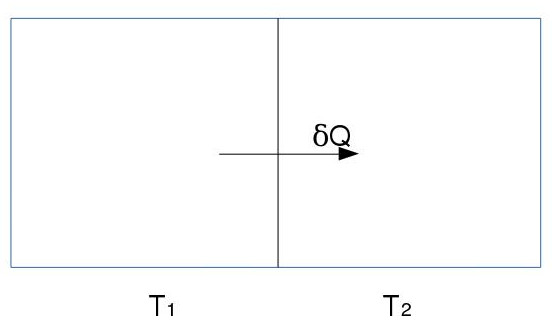
\includegraphics[width=5cm]{Bilder/Frage6.jpg} 
\end{wrapfigure}
Wärme $\delta Q$ geht spontan nur von einer höheren zu einer tieferen Temperatur. \\
$dS_1 = - \dfrac{\delta Q}{T_1} \\
dS_2 = \dfrac{\delta Q}{T_2} \\
\Delta S = dS_1 + dS_2 = \delta Q ( \dfrac{1}{T_2} -\dfrac{1}{T_1}) > 0$ \\
$\rightarrow $ Entropie erhöht sich $\rightarrow  \Delta S \geq \int_a^b \dfrac{\delta Q}{T} $ wobei Gleichgewicht bei reversiblen Prozessen.
\subsection{7}
\begin{myfrag}
Gebe die thermodynamischen Definitionen für die Freie Energie F, die
Enthalpie H, die Freie Enthalpie G und das Grosskanonische Potential $\Phi $
an. Was sind jeweils die entsprechenden Differentiale? Wie können
thermodynamische Größen und generalisierte Kräfte mit den
thermodynamischen Potentialen berechnet werden?
\end{myfrag} \quad \\
Freie Energie : $F(T,V,N) = E-TS \quad dF = -SdT -pdV+\mu dN$ \\
Enthalpie : $ H(S;p,N)=E-TS+pV \quad dH = TdS +Vdp+\mu dN$ \\
Freie Enthalpie : $ G(T;p;N)=E_TS+pV \quad dG=-SdT+Vdp+\mu dN$ \\
Großkanonisches Potential : $\Phi(T,V,\mu ) = F-\mu N \quad d \Phi = -SdT-pdV-Nd \mu $ \\[2ex]

$ F_\alpha = - \left( \dfrac{\partial E}{\partial \alpha }\right) _{S,andere \alpha} \quad a(x,y)= \left( \dfrac{\partial A}{\partial x}\right) _y \qquad b(x,y) = \left( \dfrac{\partial A}{\partial y }\right) _x$
\subsection{8}
\begin{myfrag}
Was ist eine Legendre-Transformation?
\end{myfrag}
Legendre Transformation $H= \vec{p}\vec{q}-L(\dot{\vec{q}},q)=H(p,\vec{q} )$ \\
Eine Legendre Transformation bildet aus einer Funktion $A(x,y)$ mit $ dA= a(x,y)dx +b(x,y)dy$ eine neue Funktion $B=A-ax$ mit Differential $ dB = dA - adx -xda = bdy -xda$ Das Integral ist eine Funktion von $B(a,y)$
\subsection{9}
\begin{myfrag}
Was sind intensive und extensive thermodynamische Variablen? Gebe
Beispiele.
\end{myfrag} \quad \newline
Intensive Größen 
\begin{itemize}
\item Sind unabhängig vom Ausmaß $\alpha $ des Systems (z.B. p,T,B,$\mu $)
\end{itemize}
Extensive Größen
\begin{itemize}
\item sind proportional zum Ausmaß $\alpha (E,F,G,H, \Phi , m, N, V)$
\end{itemize}
Wie erkennt man den unterschied? Man nehme zwei identische Systeme und Trenne diese mit einer Trennwand. Entfernt man die Wand dann bleiben alle intensive Größen gleich und die extensiven ändern sich.
\subsection{10}
\begin{myfrag}
Was ist die Gibbs-Duhem Relation? Leite sie her! Was besagt die Gibbs-
Duhem Relation für die Freie Enthalpie G und das Grosskanonische
Potential $\Phi$?
\end{myfrag}
Man betrachte ein System mit der Entropie $S(E,V,N)$. In einem Bruchteil $\alpha$ des Systems ist dann die Entropie $S_\alpha=S(\alpha E,\alpha V,\alpha N)$. Da die Entrope eine intensive Größe ist, gilt
\begin{align}
S=\partd{\alpha}(\alpha S)
	&=\partdd{S}{E}\partdd{\alpha E}{\alpha}+\partdd{S}{V}\partdd{\alpha V}{\alpha}+\partdd{S}{N}\partdd{\alpha N}{\alpha}\\
	&=\frac{1}{T}E+\frac{p}{T}V+\frac{\mu}{T}N\\
	&\mathrel{\Rightarrow} E=TS-pV+ \mu N
\end{align}
Dies ist die Gibbs-Duhem-Relation. Für die Gibbs'sche freie Energie bzw. das Großkanonische Potential schreibt damit man $G = E - T S + pV = \mu N$ bzw. $\Phi = E - T S - \mu N = -pV$

\section{Thermodynamische Größen}
\subsection{11}
\begin{myfrag}
Definiere die Wärmekapazitäten $C_p$ und $C_V$, die Kompressibilität $\kappa_T$, den
Ausdehnungskoeffizienten $\alpha$ und den Spannungskoeffizienten $\gamma$ als
partielle Ableitungen. Berechne $\alpha, \gamma$, $C_p$ und $C_V$ für ein ideales
klassisches Gas.
\end{myfrag}
Es gelten die Definitionen
\begin{align}
	C_p&=\left(\frac{\delta Q}{\partial T}\right)_p=T\partddd{S}{T}{p}=\partddd{E}{T}{p},\\
	C_V&=\left(\frac{\delta Q}{\partial T}\right)_V=T\partddd{S}{T}{V}=\partddd{H}{T}{V},\\
	\alpha&=\frac{1}{V}\partddd{V}{T}{p, N}=\partddd{\logn V}{T}{p, N},\\
	\kappa_T&=\frac{1}{V}\partddd{V}{p}{T}=\partddd{\logn V}{p}{T}\text{ und}\\
	\gamma&=\frac{1}{p}\partddd{p}{T}{V}=\partddd{\logn p}{T}{V}.
\end{align}
Im Idealen Gas gelten die Zustandsgleichungen $pV=Nk_BT$, $E=\frac{3}{2}Nk_BT$ und $S=Nk_B\left(\logn V+\frac{3}{2}\logn T+\mathsf{const.}\right)$. Man errechnet damit
\begin{align}
	C_p&=\partddd{E}{T}{p}=\frac{3}{2}Nk_B,\\
	C_V&=\partddd{H}{T}{V}=\partddd{E+pV}{T}{V}=\frac{5}{2}Nk_B,\\
	\alpha&=\partddd{\logn V}{T}{p, N}=\frac{1}{T},\\
	\kappa_T&=\partddd{\logn V}{p}{T}=\frac{1}{p}\text{ und}\\
	\gamma&=\partddd{\logn p}{T}{V}=\frac{1}{T}.
\end{align}

\subsection{12}
\begin{myfrag}
Leite die Umkehrrelation und die zyklische Relation für partielle
Ableitungen her.
\end{myfrag}
\begin{enumerate}[(a)]
\item Die Umkehrrelation ergibt sich direkt aus dem Satz über die Umkehrfuntion, sofern die Funktion $y(x)$ und $x(y)$ sowie ihre Ableitungen existieren.
\item TODO
\end{enumerate}
\subsection{13}
\begin{myfrag}
Zeige dass der Druck und allgemeine generalisierte Kräfte mit Hilfe einer
Ableitung der Entropie berechnet werden können.
\end{myfrag}
Sei die Kraft $f$ zum thermodynamischen Potential $\alpha$ konjugiert. Unter Verwendung der zyklischen Relation gilt
\begin{equation}
	f=\partddd{E}{\alpha}{S}\overset{\text{zykl. Rel.}}=\partddd{E}{S}{\alpha}\partddd{S}{\alpha}{E}=T\partddd{S}{\alpha}{E}
\end{equation}
\subsection{14}
\begin{myfrag}
Leite einen Ausdruck für den Spannungskoeffizienten $\gamma$ als Funktion des
Ausdehnungskoeffizienten $\alpha$ und der Kompressibilität $\kappa_T$ her.
\end{myfrag}
Nach der zyklischen Relation ist
\begin{align}
	\partddd{V}{T}{p}\partddd{T}{p}{V}&=-\partddd{V}{p}{T}\\
	V\alpha\cdot\frac{1}{p\gamma}&=-V\kappa,\\
	\Rightarrow\qquad\qquad\gamma&=-\frac{\alpha}{p\kappa}.
\end{align}
\subsection{15}
\begin{myfrag}
Leite die vier Maxwell Relationen her!
\end{myfrag}
Aus den totalen Differentialen der thermodynamischen Potentiale ergibt sich
\begin{align}
	\dif E = T \dif S - p\dif V &\Rightarrow \partddd{T}{V}{S,N}=-\partddd{p}{S}{V,N},\\
	\dif F = -S \dif T - p\dif V &\Rightarrow \partddd{S}{V}{T,N}=\partddd{p}{T}{V,N},\\
	\dif H = T \dif S - V\dif p &\Rightarrow \partddd{T}{p}{S}=\partddd{V}{S}{p}\text{ und}\\
	\dif E = -S \dif T - V\dif p &\Rightarrow \partddd{S}{p}{T}=-\partddd{V}{T}{p}.
\end{align}
\subsection{16}
\begin{myfrag}
Leite einen allgemeinen Ausdruck von physikalischen Parametern für die
Differenz zwischen den Wärmekapazitäten $C_p$ und $C_V$ her.
\end{myfrag}
Aus $\dif S = \partddd STV\dif T+\partddd SVT\dif V$ folgt durch Ableiten nach T (bei konstantem Druck)
\begin{align}
	\partddd STp &=\partddd STV\partddd TTp+\partddd SVT\partddd VTp\\
	C_p&=C_V+T\partddd SVT\partddd VTp\\
	C_p&=C_V+VT\frac{\alpha^2}{\kappa_T}
\end{align}

\subsection{17}
\begin{myfrag}
Betrachte die Druckabhängigkeit p(V) für einen adiabatischen Prozess. Leite mit
Hilfe geeigneter Relationen einen allgemeinen Ausdruck für $\partddd VpS$ her. Was ist die Adiabatengleichung unter der Annahme, dass $\sigma = \dfrac{C_p\gamma}{C_V\alpha}$ konstant bleibt? Was ist $\sigma = \dfrac{C_p\gamma}{C_V\alpha}$ für ein ideales klassisches Gas?
\end{myfrag}
TODO

\section{Kreisprozesse und Wärmekraftmaschinen}
\subsection{18}
\begin{myfrag}
Was ist mit dem Begriff reversibler Kreisprozess gemeint? Was ist die praktische
Bedeutung?
\end{myfrag}
Ein reversibler Kreisprozess ist ein Kreisprozess, der nur aus reversiblen Prozessen besteht. Praktische Bedeutung hat der Carnot-Prozess, der den maximal möglichen Wirkungsgrad realisiert. Dies kann mittels des folgenden Gedankenexperiments überprüft werden:
\begin{figure}[H]
\centering
%h\begin{tabular}{cc}
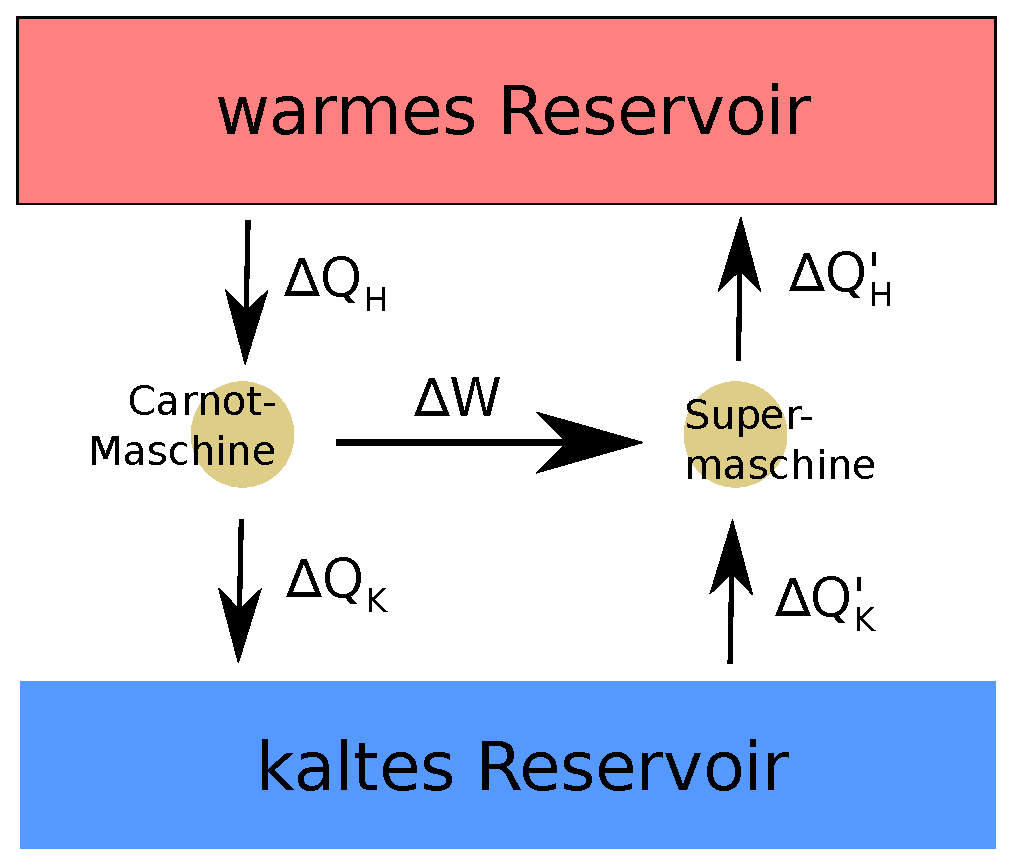
\includegraphics[width=0.45\textwidth]{Bilder/fr18.pdf}%&
\caption{Aufbau zur Bestätingung des maximalen Wirkungsgrades bei der Carnot-Maschine}
%\end{tabular}
\end{figure}
Die Carnotmaschine betreibe mit der frei werdenden Arbeit eine weitere Maschine als Wärmepumpe. Wir nehmen nun an, dass die Super-Maschine einen Wirkungsgrad $\eta>\eta_C$, des Wirkungsgrades der Carnot-Maschine habe. Dann müsste die Supermaschine mehr Wärme ins warme Reservoir transporieren, als die Carnot-Maschine verbraucht. Global heißt das, dass Wärme spontan vom kalten zum warmen Reservoir fließt, was dem zweiten Hauptsatz wiederspricht. Damit haben alle anderen reversiblen Kreisprozesse höchstens einen kleineren Wirkungsgrad. Da man dann das Experiment umdrehen und die Supermaschine zum Treiben des Stirlingmotors nutzen kann, müssen die Wirkungsgrade gleich sin.

\subsection{19}
\begin{myfrag}
Wie sind die Wirkungsgrade für Motoren, Kühlmaschinen und Wärmepumpen
definiert?
\end{myfrag}
Es gilt
\begin{align}
	\eta&=-\frac{\Delta W}{\Delta Q_H}\text{ für Motoren,}\\
	\eta_K&=-\frac{\Delta W}{\Delta Q_K}\text{ für Kältemaschinen,}\\
	\eta_W&=-\frac{\Delta W}{\Delta Q_W}\text{ für Wärmemaschinen.}
\end{align}

\subsection{20}
\begin{myfrag}

Beweise dass alle reversiblen Kreisprozesse den gleichen Wirkungsgrad haben
müssen. Wie kann man dies zu einer thermodynamischen Definition der
Temperatur nutzen?
\end{myfrag} \quad \\
\begin{wrapfigure}{r}{0.3\textwidth}
\vspace{-35mm}
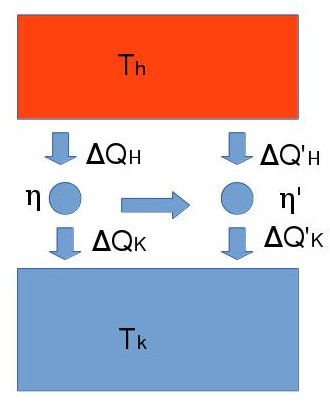
\includegraphics[width=4cm]{Bilder/Frage20.jpg} 

\end{wrapfigure}
Behauptung: Alle reversiblen Kreisprozesse haben den gleichen Wirkungsgrad.\\[2ex]
Annahme: $\eta' <\eta$ \\[2ex]
$\eta = \dfrac{|\Delta W|}{|\Delta Q_H |} \quad \eta' = \dfrac{|\Delta W|}{|\Delta Q_H' |}$ \\
$\eta' < \eta \Rightarrow \dfrac{|\Delta W|}{|\Delta Q_H' |} < \dfrac{|\Delta W|}{|\Delta Q_H |} \\ \Rightarrow | \Delta Q_H'| > | \Delta Q_H | $ \\
$\Rightarrow $ Wärme wird spontan von kalten zum heißen Reservoir überführt $\nRightarrow$ Zweiter Hauptsatz. \\[2ex]
Wirkungsgrad reversibler Kreisprozesse: \\
$\eta = 1 - \dfrac{T_K}{T_H} \qquad \dfrac{|\Delta Q_H|}{|\Delta Q_K|}$
%TODO ok ist jetzt zweimal drin...
 
\subsection{21}
\begin{myfrag}
Beschreibe den Carnot Kreisprozess und skizziere die dazugehörigen p-V und S-T
Diagramme. Berechne den Wirkungsgrad für reversible Kreisprozesse
\end{myfrag}
\begin{figure}[H]
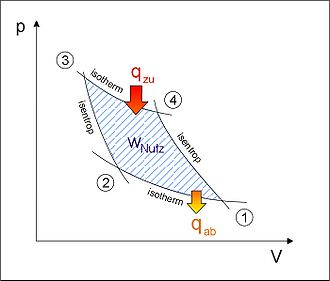
\includegraphics[width=5cm]{Bilder/Frage21pV.jpg} 
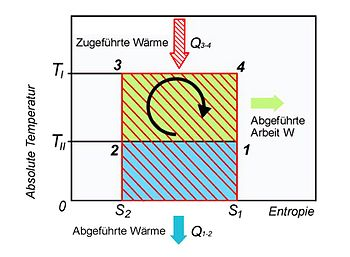
\includegraphics[width=6cm]{Bilder/Frage21TS.jpg} 
\end{figure}
Carnot
\begin{enumerate}
\item isotherme Expansion
\item adiabatische Expansion
\item isotherme Kompression
\item adiabatische Kompression
\end{enumerate}
Nach einem Durchgang gilt $ \Delta E = \Delta W + \Delta Q = 0$
\\
$\left. \begin{array}{c} \Delta Q_H = \int_1 TdS = T_H(S_b-S_a) > 0 \\ \Delta Q_K = \int_1 TdS = T_K(S_a-S_b) > 0
\end{array} \right\rbrace \Delta W + \Delta Q_H + \Delta Q_K = 0 \ \Rightarrow \ \Delta W = - \Delta Q_H - \Delta Q_K$ \\
$\Rightarrow$ \\[2ex] Arbeit wird Produziert \\

$\eta = - \dfrac{\Delta W}{ \Delta Q_H} = \dfrac{\Delta Q_H + \Delta Q_K}{\Delta Q_H}= \dfrac{T_H(S_b-S_a) + T_K(S_a -S_b)}{T_H(S_b-S_a)}=\dfrac{T_H-T_K)(S_b-S_a)}{T_H(S_b-S_a)} = 1 -\dfrac{T_K}{T_H}$


\subsection{22}
\begin{myfrag}
Beschreibe den Stirling Kreisprozess und skizziere das dazugehörige p-V
Diagramm. Wie könnte man einen realistischen Stirling Motor konstruieren?
Beschreibe eine geeignete Kolbenanordnung und die einzelnen Schritte des
Motors.
\end{myfrag}
\subsection{23}
\begin{myfrag}
Was sind wichtige Gründe, dass reale Maschinen einen geringeren Wirkungsgrad
haben? Wie kann die Entropieproduktion errechnet werden?
\end{myfrag}
\subsection{24}
\begin{myfrag}
Argumentiere, dass für effiziente Prozesse die Temperaturunterschiede beim
Überführen von Wärme möglichst klein sein sollten.
\end{myfrag}


\chapter{Statistische Mechanik}
\section{Kombinatorik}
\subsection{25}
\begin{myfrag}
\end{myfrag}
\subsection{26}
\begin{myfrag}
\end{myfrag}
\subsection{27}
\begin{myfrag}

\end{myfrag}
\subsection{28}
\begin{myfrag}
Was ist eine Wahrscheinlichkeitsverteilung? Wie werden Erwartungswerte
allgemein berechnet?
\end{myfrag} \quad \\
Jeder Mikrozustand hat eine Wahrscheinlichkeit $P_r$ bzw. $P(\{ \vec{r},\vec{p} _i \} )$ \\ Eine Dichtematrix $\rho = \sum_r P_r \left|r\right\rangle \left\langle r \right| $ ist ein Operator , der die Wahrscheinlichkeitsverteilung beschreibt. $\exists$ Basis $\left| r \right\rangle$ die $\rho $ diagonalsiert, i.A. nicht diagonale Erwartungswerte einer Größe $\Omega $ ist durch \\[1ex]
$<\Omega > = \int \Omega ( \{ \vec{r} _i , \vec{p} _i \}) P_i(\{ \vec{r} _i , \vec{p} _i \} ) d\Gamma $\\[1ex]
$<\Omega> = tr(\rho \Omega )= \sum _ r P_r \left\langle r \right| \Omega \left| r \right\rangle $ \\
Fluktuationen: \\[1ex]
$\Delta \Omega = \sqrt{\Delta \Omega ^2} = \sqrt{\left\langle (\Omega - \left\langle \Omega \right\rangle ) ^2 \right\rangle} = \sqrt{\left\langle \Omega ^2 \right\rangle - 2 \Omega \left\langle \Omega \right\rangle  + \left\langle \Omega \right\rangle ^2} = \sqrt{\left\langle \Omega ^2 \right\rangle - \left\langle \Omega \right\rangle ^2} \\ \Rightarrow \ \left\langle \Omega ^2 \right\rangle \geqslant  \left\langle \Omega \right\rangle ^2 $
\subsection{29}
\begin{myfrag}
Was besagt der zentrale Grenzwertsatz?
\end{myfrag} \quad \\
Der zentrale Grenzwertsatz besagt, dass für $ \Omega = \sum \limits_{i=1}^n y_i $ d.h. eine Summe von sehr vielen Zufallsvariablen $y_i$ mit beliebiger identischer Verteilung $P_y(y_i)$ gilt ( im Grenzwert $ n \rightarrow \infty) $ \\[1ex]
$ P (\Omega ) = \dfrac{1}{\sqrt{2 \pi}\Delta \Omega } \exp\left(- \dfrac{1}{2} \left( \dfrac{\Delta \Omega - \left\langle \Omega \right\rangle ^2}{\Delta \Omega} \right) \right)$  \qquad $ \left\langle \Omega \right\rangle  = \sum \limits_{i=0}^n \left\langle y_i \right\rangle = n \left\langle y \right\rangle $
\subsection{30}
\begin{myfrag}
Was ist die Definition der Entropie von einer allgemeinen Wahrscheinlichkeitsverteilung?
\end{myfrag}
\begin{equation}
	S=P(n)\logn P(n)
\end{equation}
\subsection{31}
\begin{myfrag}
Beschreibe das Konzept des Mikrokanonischen Ensembles. Was ist die
Wahrscheinlichkeitsverteilung im Mikrokanonischen Ensemble?
\end{myfrag}
Im Mikrokanonischen Ensemble wird angenommen, dass die Gesamtenergie und die Teilchenzahl erhalten sind, d.h. das System ist vollständig isoliert. Für die Verteilung von $n$ Energiequanten auf $N$ Oszillatoren oder ein vergleichbares Problem gilt
\begin{equation}
	Z_m=\Omega=\binkoef{N+n-1}{n}=\frac{(N+n-1)!}{(N-1)!n!}
\end{equation}
\subsection{32}
\begin{myfrag}
Mit welchem Ausdruck kann die Gesamtzahl der Zustände $\Omega$ im
Mikrokanonischen Ensemble berechnet werden? Was ist die Entropie?
\end{myfrag}
Siehe Frage 31 %TODO was zum geier???
\subsection{33}
\begin{myfrag}
Wann sind zwei Systeme im energetischen Gleichgewicht im Mikrokanonischen
Ensemble? Was bedeutet das für die Entropie?
\end{myfrag}
Die Systeme müssen die gleiche Energie haben. Die Entropie bleibt gleich. %TODO stimmt das?
\subsection{34}
\begin{myfrag}
Definiere Temperatur im Mikrokanonischen Ensemble. Wie werden
generalisierte Kräfte berechnet?
\end{myfrag}
\subsection{35}
\begin{myfrag}
Was besagen die Stabilitätsbedingungen?
\end{myfrag}
\subsection{36}
\begin{myfrag}
Leite das Ideale Gasgesetz mit Hilfe des Mikrokanonischen Ensembles her.
Zeige, dass die durchschnittliche Energie pro Teilchen E=3kT/2 ist.
\end{myfrag}
\subsection{37}
\begin{myfrag}
Betrachte ein vereinfachtes quantisiertes Modell für ein „Polymer“, wobei die
einzelnen Polymerglieder der Länge d nur nach links oder rechts zeigen können.
Berechne die generalisierte Kraft konjugiert zur Länge L mit Hilfe des
Mikrokanonischen Ensembles.
\end{myfrag}
\subsection{38}
\begin{myfrag}
Was versteht man unter dem Loschmidt Paradoxon und dem Zermelo Paradoxon?
Beschreibe einen Maxwellschen Dämon.
\end{myfrag}
\subsection{39}
\begin{myfrag}
Beschreibe das Konzept des Kanonischen Ensembles und leite es mit Hilfe des
Mikrokanonischen Ensembles her. Was ist die Boltzmann Verteilung?
\end{myfrag}
\subsection{40}
\begin{myfrag}
Was ist die kanonische Zustandssumme? Leite den Erwartungswert der Energie
als Ausdruck der Zustandssumme her.
\end{myfrag} \quad \\
Kanonische Zustandsumme: \\
$ Z= \sum \limits_r \exp ^{-\beta \epsilon _r} $ \quad \\ Zustandsintegral  $Z = \int d \Gamma \exp ^{-\beta H} $ \\[1ex]
Erwartungswert:$ \left\langle A_r \right\rangle = \dfrac{\sum _r \exp ^{-\beta \epsilon _r}}{Z}$ \\[1ex]
$\Rightarrow \left\langle E \right\rangle = \dfrac{\sum _r \epsilon _r \exp ^{-\beta \epsilon _r}}{Z} = \dfrac{\sum _r \dfrac{\partial}{\partial \beta} \exp ^{-\beta \epsilon _r}}{Z} = -\dfrac{\dfrac{\partial Z}{\partial \beta}}{Z} = - \dfrac{\partial lnZ}{\partial \beta}$
\subsection{41}
\begin{myfrag}
Wie ist die Freie Energie definiert? Wie können Energie, Entropie sowie
generalisierte Kräfte (Druck, etc.) als Funktion der Freien Energie berechnet
werden?
\end{myfrag} \quad \\
Freie Energie : $ F = -k_B T lnZ \\[1ex]
E = \dfrac{\partial (\beta F)}{\partial \beta } = - \dfrac{\partial lnZ}{\partial \beta } \\[1ex]
S= - \left( \dfrac{\partial F}{\partial T} \right) _\alpha = k_BlnZ + \dfrac{E}{T} \\[1ex]
F_\alpha =- \left( \dfrac{\partial E}{\partial \alpha } \right)_S = - \left( \dfrac{\partial F}{\partial \alpha } \right) _T \qquad p = - \left( \dfrac{\partial F}{\partial V} \right)_T \qquad m= - \left( \dfrac{\partial F}{\partial B} \right)_T$ 
\subsection{42}
\begin{myfrag}
Vergleiche die Konzepte des Kanonischen und des Mikrokanonischen Ensembles
in einer Liste: Was ist die jeweilige physikalische Situation? Was ist jeweils die
Zustandssumme und das zentrale thermodynamische Potential? Wie werden
thermodynamische Größen (gen. Kräfte, Druck, Temperatur, Energie und
Entropie) bestimmt? Was sind die Besetzungswahrscheinlichkeiten?
\end{myfrag} \quad \\
$\begin{array}{l | l}
$Mikrokan. Ensemble$ & $Kanonisches Ensemble$ \\ \hline 
$Annahme: isoliert, E = const $ & $ in thermischen Kontakt, T = const $ 
\\[1.5ex]
$Zustandsintegral $ \Omega = \int d \Gamma \delta (E-H(\{\vec{r} _i , \vec{p} _i \} )) & $ Zustandsintegral $ Z= \int d \Gamma \exp ^{-\beta H(\{ \vec{r} _i , \vec{p} _i \} ) } 
\\[1.5ex]
 $zentrales Thermodyn. Potential $ S=k:Bln \Omega & F=-k_B T ln Z 
\\
P_r = \dfrac{1}{\Omega} 
&
 P_r = \dfrac{\exp^{-\beta \epsilon _r}}{Z}
 \\[1.5ex]
\dfrac{1}{T}= \left( \dfrac{\partial S}{\partial E} \right) _{V,N} 
& 
E= - \dfrac{\partial lnZ}{\partial \beta} = \dfrac{\partial (\beta F)}{\partial
 \beta} 
\\[1.5ex]
F_\alpha = T\left( \dfrac{\partial S}{\partial \alpha } \right) _{E} & F_\alpha = - \left( \dfrac{\partial S}{\partial \alpha } \right) _{T}
\end{array} $
\subsection{43}
\begin{myfrag}
Wende die Methoden des Kanonischen Ensembles auf das Ideale Klassische Gas
an. Rechne die Erwartungswerte für den Druck, die Energie und die Entropie aus.
\end{myfrag} \quad \\
klassisches ideales Gas: \\
$Z = \int \prod \limits _{i=1}^N d^3 \vec{r} _i \prod \limits_{i=1}^N d^3 \vec{p} _i \exp ^{-\beta \sum \limits_i \dfrac{p_i^2}{2m} } \qquad $NR: $ \int dp_x dp_y dp_y \exp ^{-\beta \dfrac{p_x^2+p_y^2+p_z^2}{2m}}=(\int dy \exp ^{\alpha y^2})^3  
\\
 = V^N\left( \sqrt{\dfrac{2m \pi}{\beta}} \right) ^{3N} = V^N(2m\pi k_B T)^{\dfrac{3N}{2}} \qquad \qquad \qquad \qquad = \left( \sqrt{ \dfrac{ \pi }{\alpha }}\right) ^2
 \\
 F= -k_B TlnZ = -k_B T N (lnV + \dfrac{2}{3}lnT + const) 
 \\[1ex]
E= - \dfrac{\partial lnZ}{\partial \beta} = \dfrac{\partial N(lnV - \dfrac{2}{3}lnT + const}{\partial \beta} = \dfrac{3N}{2\beta}= \dfrac{3}{2} Nk_B T
\\[1ex]
p= -\left(\dfrac{\partial F}{\partial V} \right) _T = k_B TN \dfrac{\partial lnV}{\partial V} = \dfrac{k_B TN}{V} \quad \Rightarrow \quad pV= Nk_B T
\\[1ex]
S= \dfrac{E_F}{T} = k_BlnZ + \dfrac{E}{T} =k_B N (lnV + \dfrac{3}{2}lnT+ const)+\dfrac{3}{2} N k_B$
\subsection{44}
\begin{myfrag}
Betrachte ein vereinfachtes quantisiertes Modell für ein „Polymer“, wobei die
einzelnen Polymerglieder der Länge d nur nach links oder rechts zeigen können.
Berechne den Erwartungswert der Länge L mit Hilfe des Kanonischen Ensembles
als Funktion der Kraft (siehe auch Frage 37.).
\end{myfrag} \quad \\
$Z= \sum \limits_{Zustaende} \exp ^{-\beta H}
= \sum \limits_{r_j=\pm} \exp ^{-\beta \sum \limits_j H_j} \qquad j = 1,...,N  \quad r_j = \pm $ Zustand des Segments j$
\\[1.5ex]
H= \sum \limits_j H_j \qquad H_j = r_j Fd= \pm Fd 
\\[1.5ex]
Z = \sum \limits _{r_j = \pm } \exp ^{-\beta \sum \limits _j H_j}= \prod \limits_{j=1}^N \sum \limits _{r=\pm} \exp ^{-\beta rFd}
\\[1.5ex]
Z_1 = \sum \limits_{r=\pm} \exp ^{-\beta rFd} = \exp ^{-\beta Fd} = \exp ^{-\beta Fd} + \exp ^{\beta Fd} = 2cosh(\beta Fd)
\\[1.5ex]
L=N\left\langle l \right\rangle \qquad l=rd=\pm d \qquad \left\langle l \right\rangle = \dfrac{\sum \limits _{r=\pm} \exp ^{-\beta rFd} rd}{Z_1}
\\[1.5ex]
P_r = \dfrac{\exp ^{-\beta H_1(r)}}{Z_1} \qquad \left\langle A \right\rangle = \sum \limits _r P_r A_r = \dfrac{\sum \limits _r A_r \exp ^{-\beta H(r)}}{Z} 
\\[1.5ex]
\left\langle l \right\rangle = \dfrac{d\exp ^{-\beta Fd} -d\exp ^{\beta Fd}}{cosh(\beta Fd)} = -d \dfrac{sinh(\beta Fd)}{cosh(\beta Fd)} \qquad L= \left\langle l \right\rangle = Ndtanh(\beta Fd) 
\\[1.5ex]
$Umkehrung : $F=\dfrac{k_BT}{2d}ln\left( \dfrac{Nd-L}{Nd+L} \right) $ im Mikrokanonischen Ensemble.

\subsection{45}
\begin{myfrag}
Berechne die Mischentropie für zwei ideale Gase. Erläutere ausführlich das
Gibbssche Paradoxon und dessen Lösung.
\end{myfrag}
\subsection{46}
\begin{myfrag}
Wann sind zwei Teilsysteme unabhängig? Was passiert mit der Zustandssumme,
den Wahrscheinlichkeiten und den Erwartungswerten in diesem Fall? Was
versteht man unter einer Einteilchenzustandssumme?
\end{myfrag}
\subsection{47}
\begin{myfrag}
Argumentiere, dass die Änderung des statistischen Erwartungswertes der Energie
in Erwartungswerte für die Änderung von Wärme und Arbeit aufgeteilt werden
kann. Leite einen Zusammenhang mit Änderungen der Entropie und der
generalisierten Kräfte her.
\end{myfrag}
\subsection{48}
\begin{myfrag}
Zeige allgemein, dass Energieschwankungen im kanonischen Ensemble von der
spezifischen Wärme und der Temperatur bestimmt werden können. Wie verhalten
sich die absoluten und relativen Energiefluktuationen als Funktion von N in einem
idealen Gas?
\end{myfrag}
\subsection{49}
\begin{myfrag}
Was ist der Virialsatz? Leite ihn her!
\end{myfrag}
\subsection{50}
\begin{myfrag}
Was ist das Äquipartitionstheorem? Leite es her!
\end{myfrag}
\subsection{51}
\begin{myfrag}
Leite die Verteilung der Geschwindigkeiten in eine Richtung vx und die
Maxwellsche Geschwindigkeitsverteilung für |v| her.
\end{myfrag}
\subsection{52}
\begin{myfrag}
Berechne die Erwartungswerte $\left\langle v_x \right\rangle , \left\langle |v| \right\rangle , \left\langle v^2 \right\rangle $ und die wahrscheinlichste
Geschwindigkeit max $v_{max}$ für die Maxwellsche Geschwindigkeitsverteilung. Wie
groß ist die Fluktuation der Geschwindigkeiten?
\end{myfrag}
\subsection{53}
\begin{myfrag}
Welche zwei Bedingungen müssen gegeben sein, damit eine klassische
Näherung von Quantenfreiheitsgraden sinnvoll ist?
\end{myfrag}
\subsection{54}
\begin{myfrag}
Wie ist die thermische Wellenlänge definiert? Vergleiche mit der De-Broglie
Wellenlänge typischer Geschwindigkeiten aus der Maxwellschen
Geschwindigkeitsverteilung. Welche Bedingung muss für die Dichte gelten,
damit Quanteninterferenzeffekte vernachlässigbar sind?
\end{myfrag}
\subsection{55}
\begin{myfrag}
Berechne die Zustandssumme, den Energieerwartungswert und die
spezifische Wärme für einen harmonischen Quantenoszillator.
\end{myfrag}
\subsection{56}
\begin{myfrag}
Wie ist die Einteilchenzustandsdichte $g(\omega )$ definiert? Leite die
Einteilchenzustandsdichte für den Fall von drei-dimensionalen
Wellenvektoren mit linearer Dispersionsrelation her.
\end{myfrag}
\subsection{57}
\begin{myfrag}
Was ist das Plancksche Strahlungsgesetz? Leite es her. Was ist das
Rayleigh-Jeans Gesetz für kleine Frequenzen?
\end{myfrag}
\subsection{58}
\begin{myfrag}
Beschreibe das Einstein Modell für die spezifische Wärme von Festkörpern.
Leite den entsprechenden Ausdruck für die spezifische Wärme als Funktion
der Temperatur her. Was ist der Dulong-Petit Grenzwert für die spezifische
Wärme?
\end{myfrag}
\subsection{58}
\begin{myfrag}
Erkläre im Detail das Debye Modell für die spezifische Wärme von
Festkörpern. Was sind die wichtigen Näherungen? Definiere die Debye
Wellenvektor, Frequenz und Temperatur. Was ist das Tief- bzw.
Hochtemperaturverhalten für die spezifische Wärme als Funktion der
Temperatur?
\end{myfrag}
\subsection{59}
\begin{myfrag}
Welche Eigenschaften haben Materialen mit hoher bzw. niedriger Debye
Temperatur. Warum?
\end{myfrag}
\subsection{60}
\begin{myfrag}
Schreibe einen Ausdruck für die Einteilchen-Zustandssumme über die
quantisierten kinetischen Freiheitsgrade eines Gases. Was ist die
Hochtemperaturentwicklung der Energie und der spezifischen Wärme?
Welche Bedingung muss für die Längenskalen gelten, damit die
Hochtemperaturentwicklung gerechtfertigt ist?
\end{myfrag}
\subsection{61}
\begin{myfrag}
Was ist das Verhalten der spezifischen Wärme für die Vibrationsfreiheitsgrade
eines Molekülgases?
\end{myfrag}
\subsection{62}
\begin{myfrag}
Was ist die Zustandssumme über die quantisierten Rotationsfreiheitsgrade
eines Moleküls aus zwei verschiedenen Atomen? Berechne die
Tieftemperatur-Entwicklungen der Zustandssumme, der Energie und der
spezifischen Wärme.
\end{myfrag}
\subsection{63}
\begin{myfrag}
Erkläre wie eine Hochtemperatur-Entwicklung der Rotationszustandssumme
gemacht werden kann (die MacLaurin Summen Formel sei gegeben). Erkläre,
warum cv(T) ein Maximum als Funktion der Temperatur durchläuft.
\end{myfrag}
\subsection{64}
\begin{myfrag}
Erkläre allgemein wie sich die Eigenschaften eines diskreten Spektrums
(Entartung, Energieabstände) im Temperaturverlauf von cv(T) widerspiegeln
(mit Beispiel).
\end{myfrag}
\subsection{65}
\begin{myfrag}
Was muss bei der Zustandssumme über die quantisierten
Rotationsfreiheitsgrade eines zwei-atomigen Moleküls beachtet werden, wenn
das Molkül aus identischen Atomen besteht? Wie sieht dann die
Zustandssumme für die Fälle aus, dass der Kernspin s ganz- oder halbzahlig
ist?
\end{myfrag}
\subsection{66}
\begin{myfrag}
Was versteht man unter Ortho- und Para-Wasserstoff? Wie kann das
Verhältnis von Ortho und Para-Wasserstoff im Gleichgewicht berechnet
werden? Gegen welche Werte strebt das Verhältnis für sehr große und für
sehr kleine Temperaturen?
\end{myfrag}
\subsection{67}
\begin{myfrag}
Erkläre die Darstellung von fermionischen und bosonischen Wellenfunktionen
mit Hilfe von Besetzungszahlen. Was versteht man unter
statistischer Abstoßung bzw. Anziehung?
\end{myfrag}
\subsection{68}
\begin{myfrag}
Mache eine vereinfachte Herleitung für die Bose-Einstein und die Fermi-
Dirac Verteilungen als Summe über Besetzungszahlen eines Zustandes für
den Fall dass es kein chemisches Potential gibt.
\end{myfrag}
\subsection{69}
\begin{myfrag}
Beschreibe das Konzept des Großkanonischen Ensembles. Definiere die
großkanonische Zustandssumme, das großkanonische Potential $\Phi$, die
Fugazität z und das chemische Potential $\mu$.
\end{myfrag}
\subsection{70}
\begin{myfrag}
Wie können p, N, E und S mit Hilfe des großkanonischen Potentials $\Phi$
berechnet werden?
\end{myfrag}
\subsection{71}
\begin{myfrag}
Wende das Konzept des Großkanonischen Ensembles auf ein ideales
klassisches Gas an. Was ist z? Berechne E und p als Funktion von T, V und
N.
\end{myfrag}
\subsection{72}
\begin{myfrag}
Leite allgemeine Ausdrücke für die nichtwechselwirkenden bosonischen und
fermionischen großkanonischen Zustandssummen als Produkt über Einteilchenzustände
her. Zeige, dass die Energie und die Teilchenzahl als
Summe über Einteilchenzustände ausgedrückt werden können. Was versteht
man dementsprechend unter der Bose-Einstein und der Fermi-Dirac
Verteilung?
\end{myfrag}
\subsection{73}
\begin{myfrag}
Was ist die Entwicklung in z für die Bose-Einstein und die Fermi-Dirac
Verteilung?
\end{myfrag}
\subsection{74}
\begin{myfrag}
Leite die Einteilchen-Zustandsdichte $g(\omega )$ für ein ideales Quantengas in drei
Dimensionen her.
\end{myfrag}
\subsection{75}
\begin{myfrag}
Finde Integralausdrücke für N und E als Funktion von z und T in einem
dreidimensionalen bosonischen Quantengas. Drücke die Integrale mit Hilfe
der polylogarithmischen Funktion $g_\nu (z)$  aus. Wie kann mit Hilfe dieser
Ausdrücke E als Funktion von N, V und T bestimmt werden (Eine Skizze ist
hilfreich hier).
\end{myfrag}
\subsection{76}
\begin{myfrag}
Zeige für ein dreidimensionales Quantengas, wie der Druck mit dem
Energieerwartungswert zusammenhängt.
\end{myfrag}
\subsection{77}
\begin{myfrag}
Erkläre das Konzept der Virialentwicklung am Beispiel eines idealen
Bosonen Gases. Berechne den ersten Koeffizienten.
\end{myfrag}
\subsection{78}
\begin{myfrag}
Argumentiere dass in der Berechnung der Teilchenzahl der Grundzustand
eines Bosonen Gases ab einer kritischen Temperatur gesondert behandelt
werden muss. Was ist die kritische Temperatur  $T_C$ ?
\end{myfrag}
\subsection{79}
\begin{myfrag}
Berechne den Kondensatsanteil x in einem dreidimensionalen Bosonengas als
Funktion der Temperatur und der Kondensationstemperatur $T_C$.
\end{myfrag}
\subsection{80}
\begin{myfrag}
Berechne die Energie und die spezifische Wärme in einem idealen Bose-Gas
als Funktion der Temperatur bei gegebener Dichte (d.h. gegebener kritische
Temperatur Tc). Zeichne den ungefähren Verlauf der spezifischen Wärme CV
als Funktion von T eines bosonischen Gases.
\end{myfrag}
\subsection{81}
\begin{myfrag}
Argumentiere, dass in einem Bosegas für T<Tc der Druck proportional zu $T^{\dfrac{5}{2}}$
ist.
\end{myfrag}
\subsection{82}
\begin{myfrag}
Wie ändert sich das großkanonische Ensemble falls innere Freiheitsgrade
(z.B. Spin) berücksichtigt werden müssen? Was ist der Effekt für die
Quantenstatistik und Virialentwicklung falls es entartete innere Freiheitsgrade
gibt?
\end{myfrag}
\subsection{83}
\begin{myfrag}
Wie kann man bei einem bosonischen Gas Wechselwirkungseffekte durch
einen Molekularfeldansatz (MFT) berücksichtigen?
\end{myfrag}
\subsection{84}
\begin{myfrag}
Wende das großkanonische Ensemble auf ein bosonisches Photonengas mit
Entartung g=2 und $Ek=\hbar kc$ an. Berechne die Erwartungswerte der Energie,
der Teilchenzahl und des Druckes (mit Hilfe einer Integraltabelle). Warum
gibt es keine Bose-Einstein Kondensation in diesem Fall?
\end{myfrag}
\subsection{85}
\begin{myfrag}
Was sind die Ausdrücke für die Teilchenzahl und die Energie eines
dreidimensionalen fermionischen Gases als Funktion der Fugazität?
\end{myfrag}
\subsection{86}
\begin{myfrag}
Was ist die Virialentwicklung für ein ideales Fermionengas bis zur 1.
Ordnung?
\end{myfrag}
\subsection{87}
\begin{myfrag}
Wie ist die Fermi Energie $\epsilon _F$ definiert? Berechne den Druck und die Energie
für ein ideales dreidimensionales Fermigas bei T=0 als Funktion von N, V
und $\epsilon _F$.
\end{myfrag}
\subsection{88}
\begin{myfrag}
Was ist die Sommerfeld Entwicklung? Leite sie her. Stelle die Koeffizienten als
dimensionslose Integrale dar.
\end{myfrag}
\subsection{89}
\begin{myfrag}
Wende die Sommerfeld Entwicklung auf ein ideales Fermionen Gas in drei Dimensionen
an, um die Korrekturen für kleine Temperaturen zum chemischen Potential und zur
spezifischen Wärme zu bestimmen.
\end{myfrag}
\subsection{90}
\begin{myfrag}
Wie hängt der Entwicklungsparameter $k_B T/\epsilon_F$ in der Sommerfeld Entwicklung mit dem
Parameter $\lambda^3 N/gV$ 3 N/gV zusammen (für ein ideales Fermigas)?
\end{myfrag}
\subsection{91}
\begin{myfrag}
Was besagt die Boltzmann Transport Gleichung und der Stoßzahlansatz? Erläutere die
Herleitung.
\end{myfrag}
\subsection{92}
\begin{myfrag}
Erläutere wie man einen Phasenübergang zwischen einer geordneten und einer
ungeordneten Phase quantitativ verstehen kann indem man die Freie Energie minimiert.
Was bedeutet dies für die Energie und Entropie bei hohen bzw. tiefen Temperaturen?
\end{myfrag}
\subsection{93}
\begin{myfrag}
Was ist die Ehrenfest Klassifikation? Was zeichnet einen Phasenübergang von 1.
Ordnung aus? Was versteht man unter einem Ordnungsparameter?
\end{myfrag}
\subsection{94}
\begin{myfrag}
Was besagt die Gibbssche Phasenregel für die Koexistenz verschiedener Phasen?
\end{myfrag}


\end{document}